\documentclass[11pt]{article}

\usepackage{amsmath,amssymb,mathtools}
\usepackage[margin=0.85in]{geometry}
\usepackage{booktabs}
\usepackage{array}
\usepackage{enumitem}
\usepackage{tikz}
\usetikzlibrary{arrows.meta,calc,positioning}
\usepackage[hidelinks]{hyperref}

\newcommand{\R}{\mathbb{R}}
\newcommand{\Om}{\Omega}
\newcommand{\dd}{\,\mathrm{d}}
\newcommand{\V}{\mathcal{V}}
\newcommand{\Vh}{\mathcal{V}_h}
\newcommand{\Th}{\mathcal{T}_h}
\newcommand{\Pp}{\mathbb{P}}
\newcommand{\bU}{\mathbf{U}}
\newcommand{\bV}{\mathbf{V}}
\newcommand{\bK}{\mathbf{K}}
\newcommand{\bF}{\mathbf{F}}
\newcommand{\bKe}{\mathbf{K}^{e}}
\newcommand{\bFe}{\mathbf{F}^{e}}
\newcommand{\phihat}{\widehat{\phi}}

\setlength{\parindent}{0pt}
\setlength{\parskip}{0.42em}
\setlist{nosep,leftmargin=*}
\allowdisplaybreaks[1]

\begin{document}

\begin{center}
{\Large\bfseries The Finite Element Method in One Dimension}\\[4pt]
{\large ME/BME 736 -- Advanced Finite Element Methods}\\[2pt]
{\normalsize Prashant K. Jha}
\end{center}

\hrule
\vspace{0.8em}

This handout develops the one-dimensional finite element method in detail. The
starting point is a variational problem of the type already developed in the
preceding course material. The emphasis here is on the new finite element
ideas: Galerkin approximation, meshes, local polynomial basis functions,
local and global node numbering, construction of linear and higher-order
basis functions, the reference element, element matrices and vectors,
local-to-global assembly, and numerical quadrature.

The one-dimensional setting is useful because every step of the construction
can be written explicitly and visualized. The same structure will later carry
over to finite elements in two and three dimensions.

\section{Starting point: a one-dimensional variational problem}

Consider
\begin{equation}
-\frac{\dd}{\dd x}\left(a(x)\frac{\dd u}{\dd x}\right)
+c(x)u=f(x),\qquad x\in(0,L),
\label{eq:strong}
\end{equation}
with
\[
u(0)=0,
\qquad
a(L)u'(L)=q_L.
\]
Assume $a(x)>0$ and $c(x)\geq0$. The corresponding variational problem is
\begin{equation}
\boxed{
\text{find }u\in\V\text{ such that }
B(u,v)=F(v)\qquad\forall v\in\V,
}
\label{eq:weak}
\end{equation}
where
\[
\V=\{v\in H^1(0,L):v(0)=0\},
\]
\begin{align}
B(u,v)
&=\int_0^L\left[a(x)u'(x)v'(x)+c(x)u(x)v(x)\right]\dd x,
\label{eq:B}\\
F(v)
&=\int_0^L f(x)v(x)\dd x+q_Lv(L).
\label{eq:F}
\end{align}
The exact solution belongs to the infinite-dimensional space $\V$. The goal
is to replace this problem by one involving only finitely many unknown
coefficients.

\paragraph{Axial-bar specialization.}
For a one-dimensional elastic bar,
\[
a(x)=A(x)E(x),\qquad c(x)=0,
\]
where $A$ is the cross-sectional area and $E$ is Young's modulus. The unknown
$u$ is the axial displacement. If $P$ is an end load at $x=L$, then $q_L=P$.
Thus
\[
B(u,v)=\int_0^L AE\,u'v'\,\dd x,
\qquad
F(v)=\int_0^L fv\,\dd x+Pv(L).
\]
This bar problem will be used repeatedly below.

\section{Galerkin approximation before finite elements}

Let $\V_N\subset\V$ be an $N$-dimensional space spanned by known basis
functions $\psi_1,\ldots,\psi_N$:
\[
\V_N=\operatorname{span}\{\psi_1,\ldots,\psi_N\}.
\]
The Galerkin approximation seeks
\[
u_N(x)=\sum_{j=1}^N U_j\psi_j(x)
\]
such that
\begin{equation}
B(u_N,v_N)=F(v_N)
\qquad\forall v_N\in\V_N.
\label{eq:galerkin}
\end{equation}
Writing
\[
v_N(x)=\sum_{i=1}^N V_i\psi_i(x)
\]
and using bilinearity of $B$ and linearity of $F$ gives
\[
\sum_{i=1}^N V_i
\left[
\sum_{j=1}^N B(\psi_j,\psi_i)U_j-F(\psi_i)
\right]=0.
\]
Because the coefficients $V_i$ are arbitrary,
\[
\sum_{j=1}^N B(\psi_j,\psi_i)U_j=F(\psi_i),
\qquad i=1,\ldots,N.
\]
Define
\[
K_{ij}=B(\psi_j,\psi_i),
\qquad
F_i=F(\psi_i).
\]
Then
\begin{equation}
\boxed{\bK\bU=\bF.}
\label{eq:global-galerkin}
\end{equation}
The unknown function has therefore been replaced by $N$ unknown coefficients.

\subsection*{Why an arbitrary Galerkin basis is not yet a finite element basis}

The basis functions $\psi_i$ could be global functions such as polynomials or
trigonometric functions. Such functions are generally nonzero over most or all
of the domain. Consequently $B(\psi_j,\psi_i)$ is usually nonzero for many
pairs $(i,j)$ and $\bK$ is dense.

The finite element method keeps the Galerkin idea but constructs basis
functions that are nonzero only on small parts of the domain. This
\emph{local support} is the key structural difference.

\subsection*{A simple global Galerkin example}

For a uniform axial bar with constant $AE$, no distributed load, $u(0)=0$,
and end load $P$, the exact solution is
\[
u(x)=\frac{P}{AE}x.
\]
Take $\psi_1(x)=1$ and $\psi_2(x)=x$. Then
\[
u_N=U_1+U_2x.
\]
The essential condition gives $U_1=0$. The Galerkin equation then yields
\[
AE\,U_2L=PL,
\qquad
U_2=\frac{P}{AE},
\]
so this space happens to contain the exact solution. The example is useful,
but these basis functions are global. FEM will instead construct basis
functions from a mesh.

\section{Mesh, elements, nodes, and the finite element basis}

\subsection{Partition of the interval}

Let
\[
0=x_1<x_2<\cdots<x_N=L
\]
be global nodes. The domain is partitioned into elements
\[
\Om^e=[x_1^e,x_2^e],\qquad e=1,\ldots,N_e,
\]
where neighboring elements share endpoint nodes. For a linear three-element
mesh,
\[
\Om^1=[x_1,x_2],\qquad
\Om^2=[x_2,x_3],\qquad
\Om^3=[x_3,x_4].
\]

\begin{center}
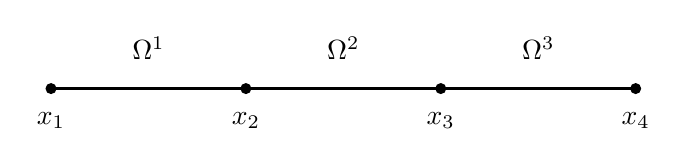
\begin{tikzpicture}[x=1.65cm,y=1cm]
\draw[thick] (0,0)--(4.5,0);
\foreach \x/\lab in {0/$x_1$,1.5/$x_2$,3/$x_3$,4.5/$x_4$}{
  \fill (\x,0) circle (2pt); \node[below=5pt] at (\x,0) {\lab};}
\node[above=7pt] at (0.75,0) {$\Om^1$};
\node[above=7pt] at (2.25,0) {$\Om^2$};
\node[above=7pt] at (3.75,0) {$\Om^3$};
\end{tikzpicture}
\end{center}

The element length is
\[
h^e=x_2^e-x_1^e.
\]
The collection of all elements is the mesh $\Th$.

\subsection{Three requirements for nodal finite element basis functions}

The lecture construction can be summarized by three requirements.

\begin{enumerate}
\item \textbf{Polynomial on each element.}
      On an element $\Om^e$, the restriction of a basis function is a
      polynomial of prescribed degree $p^e$.
\item \textbf{Continuous across element boundaries.}
      For the $H^1$-conforming finite elements considered here, neighboring
      polynomial pieces join continuously at shared nodes.
\item \textbf{Nodal interpolation property.}
      The global basis function $\phi_i$ associated with global node $x_i$
      satisfies
      \begin{equation}
      \phi_i(x_j)=\delta_{ij}.
      \label{eq:nodal-property}
      \end{equation}
\end{enumerate}

These conditions create basis functions tied directly to the mesh rather than
to the whole domain.

\subsection{Begin with one two-node linear element}

Consider one element
\[
\Om^e=[x_1^e,x_2^e].
\]
A linear element has two local nodes and therefore two local basis functions.
Let
\[
\phi_1^e(x)=a_1+b_1x,
\qquad
\phi_2^e(x)=a_2+b_2x.
\]
The nodal conditions are
\[
\phi_1^e(x_1^e)=1,\qquad \phi_1^e(x_2^e)=0,
\]
\[
\phi_2^e(x_1^e)=0,\qquad \phi_2^e(x_2^e)=1.
\]
Solving these two small interpolation problems gives
\begin{equation}
\boxed{
\phi_1^e(x)=\frac{x_2^e-x}{h^e},
\qquad
\phi_2^e(x)=\frac{x-x_1^e}{h^e}.}
\label{eq:linear-local-basis}
\end{equation}
Thus
\[
\phi_a^e(x_b^e)=\delta_{ab},\qquad a,b=1,2.
\]

\begin{center}
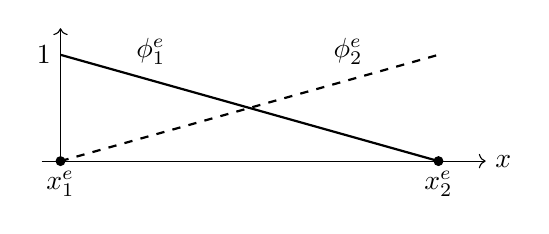
\begin{tikzpicture}[x=2.4cm,y=1.35cm]
\draw[->] (-0.1,0)--(2.25,0) node[right] {$x$};
\draw[->] (0,-0.05)--(0,1.25);
\draw[thick] (0,1)--(2,0);
\draw[thick,dashed] (0,0)--(2,1);
\fill (0,0) circle (1.8pt); \fill (2,0) circle (1.8pt);
\node[below] at (0,0) {$x_1^e$}; \node[below] at (2,0) {$x_2^e$};
\node[left] at (0,1) {$1$};
\node[above right] at (0.35,0.82) {$\phi_1^e$};
\node[above left] at (1.65,0.82) {$\phi_2^e$};
\end{tikzpicture}
\end{center}

The two functions form a local basis on the element. A finite element function
restricted to this element has the form
\begin{equation}
u_h|_{\Om^e}=U_1^e\phi_1^e+U_2^e\phi_2^e.
\label{eq:local-linear-interpolation}
\end{equation}
Because of the nodal property,
\[
u_h(x_1^e)=U_1^e,
\qquad
u_h(x_2^e)=U_2^e.
\]

\subsection{Patching local linear functions into global basis functions}

Now return to the three-element, four-node mesh. Each global basis function is
constructed by combining the appropriate local linear pieces and setting the
function to zero elsewhere.

For example,
\[
\phi_1(x)=
\begin{cases}
\phi_1^1(x), & x\in\Om^1,\\
0, & \text{otherwise},
\end{cases}
\]
while the basis function associated with the shared node $x_2$ is
\[
\phi_2(x)=
\begin{cases}
\phi_2^1(x), & x\in\Om^1,\\
\phi_1^2(x), & x\in\Om^2,\\
0, & \text{otherwise}.
\end{cases}
\]
Similarly,
\[
\phi_3(x)=
\begin{cases}
\phi_2^2(x), & x\in\Om^2,\\
\phi_1^3(x), & x\in\Om^3,\\
0, & \text{otherwise},
\end{cases}
\qquad
\phi_4(x)=
\begin{cases}
\phi_2^3(x), & x\in\Om^3,\\
0, & \text{otherwise}.
\end{cases}
\]

\begin{center}
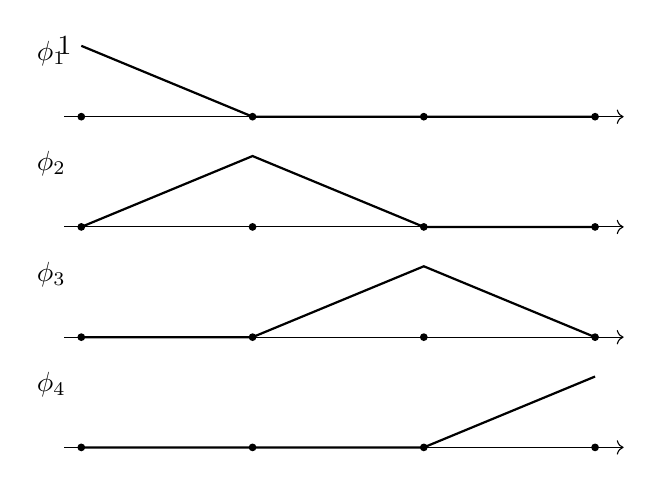
\begin{tikzpicture}[x=1.45cm,y=1.0cm]
\foreach \r/\i in {0/1,-1.4/2,-2.8/3,-4.2/4}{
  \draw[->] (-0.15,\r)--(4.75,\r);
  \foreach \x in {0,1.5,3,4.5}{\fill (\x,\r) circle (1.4pt);}
  \node[left] at (-0.05,\r+0.8) {$\phi_{\i}$};
}
\draw[thick] (0,0.9)--(1.5,0)--(4.5,0);
\draw[thick] (0,-1.4)--(1.5,-0.5)--(3,-1.4)--(4.5,-1.4);
\draw[thick] (0,-2.8)--(1.5,-2.8)--(3,-1.9)--(4.5,-2.8);
\draw[thick] (0,-4.2)--(3,-4.2)--(4.5,-3.3);
\node[left] at (0,0.9) {$1$};
\end{tikzpicture}
\end{center}

The diagrams make two important properties visible:
\begin{itemize}
\item $\phi_i(x_j)=\delta_{ij}$;
\item each $\phi_i$ is nonzero only on the element or elements touching node
      $x_i$.
\end{itemize}
The second property is the local support responsible for sparsity.

The global linear finite element space is
\[
\Vh
=
\{v_h\in C([0,L]):v_h|_{\Om^e}\in\Pp_1(\Om^e)
\text{ for each }e\}.
\]
Every $u_h\in\Vh$ can be written
\begin{equation}
u_h(x)=\sum_{i=1}^{N}U_i\phi_i(x).
\label{eq:global-expansion}
\end{equation}
Using \eqref{eq:nodal-property},
\[
u_h(x_j)=\sum_i U_i\phi_i(x_j)=U_j.
\]
Therefore the coefficients are the nodal values of the finite element
function.

\section{Higher-order elements}

The same construction extends naturally when each element contains more than
two nodes.

\subsection{A three-node quadratic element}

Consider one element with local nodes
\[
x_1^e<x_2^e<x_3^e.
\]
A quadratic element has three local basis functions. Each is a polynomial of
degree at most two and satisfies
\[
\phi_a^e(x_b^e)=\delta_{ab},\qquad a,b=1,2,3.
\]
For example, the first function is the unique quadratic satisfying
\[
\phi_1^e(x_1^e)=1,
\qquad
\phi_1^e(x_2^e)=0,
\qquad
\phi_1^e(x_3^e)=0.
\]
The three functions can be written directly using Lagrange interpolation:
\begin{align}
\phi_1^e(x)
&=\frac{(x-x_2^e)(x-x_3^e)}{(x_1^e-x_2^e)(x_1^e-x_3^e)},\\
\phi_2^e(x)
&=\frac{(x-x_1^e)(x-x_3^e)}{(x_2^e-x_1^e)(x_2^e-x_3^e)},\\
\phi_3^e(x)
&=\frac{(x-x_1^e)(x-x_2^e)}{(x_3^e-x_1^e)(x_3^e-x_2^e)}.
\label{eq:quadratic-physical}
\end{align}

\begin{center}
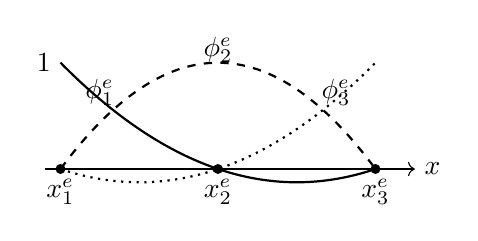
\begin{tikzpicture}[x=2.0cm,y=1.35cm]
\draw[->] (-0.1,0)--(2.25,0) node[right] {$x$};
\foreach \x/\lab in {0/$x_1^e$,1/$x_2^e$,2/$x_3^e$}{\fill (\x,0) circle (1.8pt);\node[below] at (\x,0){\lab};}
\draw[thick,domain=0:2,samples=60] plot (\x,{0.5*(\x-1)*(\x-2)});
\draw[thick,dashed,domain=0:2,samples=60] plot (\x,{\x*(2-\x)});
\draw[thick,dotted,domain=0:2,samples=60] plot (\x,{0.5*\x*(\x-1)});
\node at (0.25,0.72) {$\phi_1^e$};
\node at (1.0,1.12) {$\phi_2^e$};
\node at (1.75,0.72) {$\phi_3^e$};
\node[left] at (0,1) {$1$};
\end{tikzpicture}
\end{center}

The endpoint basis functions are not simply straight lines anymore. They may
also take negative values inside the element. What remains essential is the
nodal interpolation property and polynomial degree.

\subsection{Three quadratic elements and seven global nodes}

For three quadratic elements, neighboring elements share only their endpoint
nodes. A typical uniform mesh has
\[
\Om^1=[x_1,x_3],\qquad
\Om^2=[x_3,x_5],\qquad
\Om^3=[x_5,x_7],
\]
with midpoint nodes $x_2,x_4,x_6$.

\begin{center}
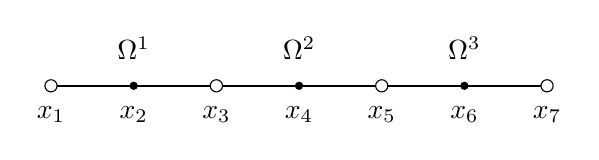
\begin{tikzpicture}[x=1.05cm,y=1cm]
\draw[thick] (0,0)--(6,0);
\foreach \x/\lab in {0/$x_1$,1/$x_2$,2/$x_3$,3/$x_4$,4/$x_5$,5/$x_6$,6/$x_7$}{
  \ifodd\numexpr\x\relax\fill (\x,0) circle (1.5pt);\else\filldraw[fill=white] (\x,0) circle (2.2pt);\fi
  \node[below=4pt] at (\x,0){\lab};}
\node[above=6pt] at (1,0) {$\Om^1$};
\node[above=6pt] at (3,0) {$\Om^2$};
\node[above=6pt] at (5,0) {$\Om^3$};
\end{tikzpicture}
\end{center}

The local-to-global node connectivity is
\[
I^1=(1,2,3),\qquad
I^2=(3,4,5),\qquad
I^3=(5,6,7).
\]
The seven global basis functions are again obtained by patching local
quadratic pieces. The midpoint functions are supported on one element; basis
functions associated with shared element endpoints are supported on two
neighboring elements.

\begin{center}
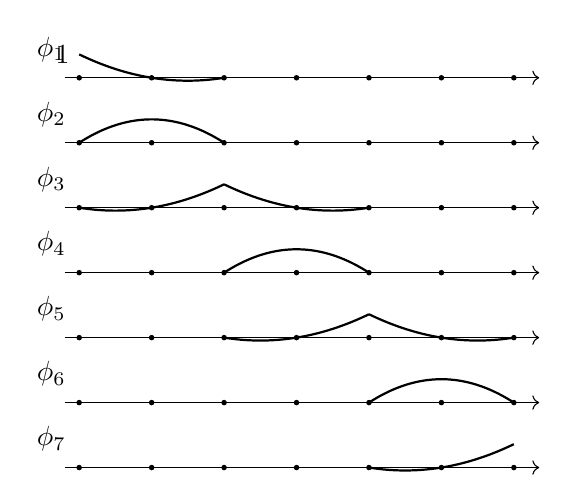
\begin{tikzpicture}[x=0.92cm,y=0.66cm]
% row 1 phi1
\foreach \r/\lab in {0/$\phi_1$,-1.25/$\phi_2$,-2.5/$\phi_3$,-3.75/$\phi_4$,-5/$\phi_5$,-6.25/$\phi_6$,-7.5/$\phi_7$}{
  \draw[->] (-0.2,\r)--(6.35,\r);
  \foreach \x in {0,1,2,3,4,5,6}{\fill (\x,\r) circle (1pt);}
  \node[left] at (-0.05,\r+0.55){\lab};
}
% basis functions on uniform quadratic mesh: each element length 2, midpoint spacing 1
\draw[thick,domain=0:2,samples=40] plot (\x,{0.45*(0.5*(\x-1)*(\x-2))});
\draw[thick,domain=0:2,samples=40] plot (\x,{-1.25+0.45*(\x*(2-\x))});
\draw[thick,domain=0:2,samples=40] plot (\x,{-2.5+0.45*(0.5*\x*(\x-1))});
\draw[thick,domain=2:4,samples=40] plot (\x,{-2.5+0.45*(0.5*(\x-3)*(\x-4))});
\draw[thick,domain=2:4,samples=40] plot (\x,{-3.75+0.45*((\x-2)*(4-\x))});
\draw[thick,domain=2:4,samples=40] plot (\x,{-5+0.45*(0.5*(\x-2)*(\x-3))});
\draw[thick,domain=4:6,samples=40] plot (\x,{-5+0.45*(0.5*(\x-5)*(\x-6))});
\draw[thick,domain=4:6,samples=40] plot (\x,{-6.25+0.45*((\x-4)*(6-\x))});
\draw[thick,domain=4:6,samples=40] plot (\x,{-7.5+0.45*(0.5*(\x-4)*(\x-5))});
\node[left] at (0,0.45) {$1$};
\end{tikzpicture}
\end{center}

This picture is the higher-order analogue of the linear hat-function picture.
The shapes differ, but the construction rules are unchanged.

\subsection{General polynomial degree}

A degree-$p$ one-dimensional Lagrange element has $p+1$ local nodes and
$p+1$ local basis functions. On each element the basis functions are
polynomials of degree at most $p$, they join continuously at shared endpoint
nodes, and they satisfy the nodal property. The global finite element space is
\begin{equation}
\Vh^p
=
\{v_h\in C([0,L]):v_h|_{\Om^e}\in\Pp_p(\Om^e)
\text{ for every }e\}.
\label{eq:Vhp}
\end{equation}

\section{The reference or master element}

Constructing new polynomial formulas separately on every physical element is
unnecessary. Every one-dimensional element can be related to one fixed
reference element
\[
\widehat\Om=[-1,1],
\]
with coordinate $\xi$.

\subsection{Coordinate mapping}

For the physical element
\[
\Om^e=[x_1^e,x_2^e],
\qquad
h^e=x_2^e-x_1^e,
\]
seek a linear map $x^e(\xi)=m\xi+c$ such that
\[
x^e(-1)=x_1^e,
\qquad
x^e(1)=x_2^e.
\]
Solving gives
\begin{equation}
\boxed{
x^e(\xi)
=\frac{x_1^e+x_2^e}{2}
+\frac{h^e}{2}\xi.}
\label{eq:map}
\end{equation}
The inverse map is
\begin{equation}
\boxed{
\xi^e(x)
=\frac{2}{h^e}
\left(x-\frac{x_1^e+x_2^e}{2}\right).}
\label{eq:inverse-map}
\end{equation}
The Jacobians are
\begin{equation}
J_x^e=\frac{\dd x^e}{\dd\xi}=\frac{h^e}{2},
\qquad
J_\xi^e=\frac{\dd\xi^e}{\dd x}=\frac{2}{h^e}
=\frac{1}{J_x^e}.
\label{eq:jacobians}
\end{equation}

\begin{center}
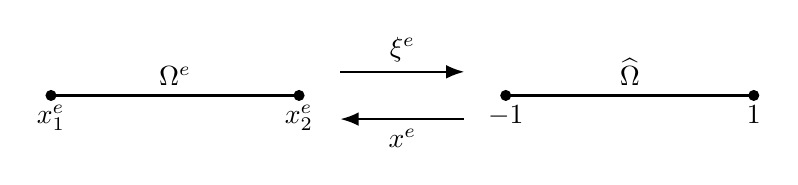
\begin{tikzpicture}[x=1.05cm,y=1cm,>=Latex]
\draw[thick] (0,0)--(3,0); \fill (0,0) circle (2pt); \fill (3,0) circle (2pt);
\node[below] at (0,0) {$x_1^e$}; \node[below] at (3,0) {$x_2^e$};
\node[above] at (1.5,0) {$\Om^e$};
\draw[->,thick] (3.5,0.3)--(5.0,0.3) node[midway,above] {$\xi^e$};
\draw[<-,thick] (3.5,-0.3)--(5.0,-0.3) node[midway,below] {$x^e$};
\draw[thick] (5.5,0)--(8.5,0); \fill (5.5,0) circle (2pt); \fill (8.5,0) circle (2pt);
\node[below] at (5.5,0) {$-1$}; \node[below] at (8.5,0) {$1$};
\node[above] at (7,0) {$\widehat\Om$};
\end{tikzpicture}
\end{center}

\subsection{Lagrange basis functions on the master element}

For degree $p$, choose $p+1$ distinct master-element nodes
\[
\xi_1,\ldots,\xi_{p+1}.
\]
The local reference basis function associated with node $i$ is
\begin{equation}
\boxed{
\widehat\phi_i(\xi)
=
\prod_{\substack{k=1\\k\neq i}}^{p+1}
\frac{\xi-\xi_k}{\xi_i-\xi_k}.}
\label{eq:lagrange}
\end{equation}
At a reference node $\xi_j$, every factor is finite and the numerator contains
$\xi_j-\xi_j=0$ unless $i=j$. Hence
\begin{equation}
\widehat\phi_i(\xi_j)=\delta_{ij}.
\label{eq:ref-nodal}
\end{equation}

For $p=1$, with nodes $-1$ and $1$,
\[
\widehat\phi_1(\xi)=\frac{1-\xi}{2},
\qquad
\widehat\phi_2(\xi)=\frac{1+\xi}{2}.
\]
For $p=2$, with nodes $-1,0,1$,
\begin{equation}
\widehat\phi_1(\xi)=\frac12\xi(\xi-1),
\qquad
\widehat\phi_2(\xi)=1-\xi^2,
\qquad
\widehat\phi_3(\xi)=\frac12\xi(\xi+1).
\label{eq:quadratic-reference}
\end{equation}

\begin{center}
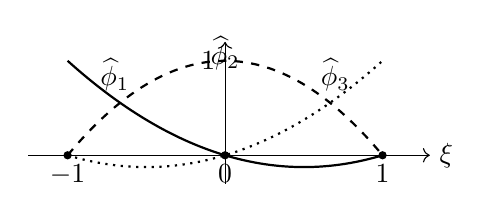
\begin{tikzpicture}[x=2.0cm,y=1.2cm]
\draw[->] (-1.25,0)--(1.3,0) node[right] {$\xi$};
\draw[->] (0,-0.3)--(0,1.2);
\foreach \x/\lab in {-1/$-1$,0/$0$,1/$1$}{\fill (\x,0) circle (1.5pt);\node[below] at (\x,0){\lab};}
\draw[thick,domain=-1:1,samples=60] plot (\x,{0.5*\x*(\x-1)});
\draw[thick,dashed,domain=-1:1,samples=60] plot (\x,{1-\x*\x});
\draw[thick,dotted,domain=-1:1,samples=60] plot (\x,{0.5*\x*(\x+1)});
\node at (-0.7,0.85) {$\widehat\phi_1$};
\node at (0,1.08) {$\widehat\phi_2$};
\node at (0.7,0.85) {$\widehat\phi_3$};
\node[left] at (0,1) {$1$};
\end{tikzpicture}
\end{center}

The physical-element basis functions are obtained by composition:
\begin{equation}
\phi_i^e(x)=\widehat\phi_i(\xi^e(x)).
\label{eq:physical-basis}
\end{equation}
The derivative follows from the chain rule:
\begin{equation}
\frac{\dd\phi_i^e}{\dd x}
=
\frac{\dd\widehat\phi_i}{\dd\xi}
\frac{\dd\xi^e}{\dd x}
=
J_\xi^e\frac{\dd\widehat\phi_i}{\dd\xi}.
\label{eq:derivative-transform}
\end{equation}

\subsection{Local and global node numbering}

The element formulas use local numbers $1,\ldots,p+1$, while the mesh uses
global node numbers. A connectivity table provides the correspondence.

For three linear elements,
\[
\begin{array}{c|cc}
\text{element} & \text{local node 1} & \text{local node 2}\\\hline
1&1&2\\
2&2&3\\
3&3&4
\end{array}
\]
For three quadratic elements,
\[
\begin{array}{c|ccc}
\text{element} & \text{local node 1} & \text{local node 2} & \text{local node 3}\\\hline
1&1&2&3\\
2&3&4&5\\
3&5&6&7
\end{array}
\]
If $I=I^e(a)$ denotes the global node corresponding to local node $a$ of
element $e$, then on that element
\begin{equation}
\phi_I|_{\Om^e}=\phi_a^e.
\label{eq:local-global-restriction}
\end{equation}

\section{The finite element variational problem}

Let $\V_{h,0}\subset\V$ be the finite element space satisfying the homogeneous
essential boundary condition. The finite element problem is
\begin{equation}
\boxed{
\text{find }u_h\in\V_{h,0}\text{ such that }
B(u_h,v_h)=F(v_h)
\qquad\forall v_h\in\V_{h,0}.}
\label{eq:discrete}
\end{equation}
Write
\[
u_h=\sum_{j=1}^N U_j\phi_j,
\qquad
v_h=\sum_{i=1}^N V_i\phi_i.
\]
Exactly as in the Galerkin derivation,
\[
\sum_{j=1}^N B(\phi_j,\phi_i)U_j=F(\phi_i),
\qquad i=1,\ldots,N.
\]
Thus
\[
K_{ij}=B(\phi_j,\phi_i),
\qquad
F_i=F(\phi_i),
\qquad
\boxed{\bK\bU=\bF.}
\]
The important difference from a generic global Galerkin basis is that each
$\phi_i$ has local support. Therefore most pairs of basis functions do not
overlap and most $K_{ij}$ vanish.

\section{Element matrices and element load vectors}

Because a global basis function is nonzero only on a few elements, every
global integral can be decomposed into element integrals. For an element
$\Om^e$ with local basis functions $\phi_a^e$, define
\begin{align}
K_{ab}^e
&=
\int_{\Om^e}
\left[
a(x)\frac{\dd\phi_b^e}{\dd x}
\frac{\dd\phi_a^e}{\dd x}
+c(x)\phi_b^e\phi_a^e
\right]\dd x,
\label{eq:element-K}\\
F_a^e
&=
\int_{\Om^e}f(x)\phi_a^e(x)\dd x.
\label{eq:element-F}
\end{align}
These are the local element stiffness matrix and load vector. Natural boundary
terms are added to the appropriate global load entry.

\subsection*{Two-node linear bar element}

For $a=AE$, $c=0$, and a two-node linear element,
\[
\frac{\dd\phi_1^e}{\dd x}=-\frac1{h^e},
\qquad
\frac{\dd\phi_2^e}{\dd x}=\frac1{h^e}.
\]
Hence
\begin{equation}
\boxed{
\bKe
=
\frac{A_eE_e}{h^e}
\begin{bmatrix}
1&-1\\
-1&1
\end{bmatrix}.}
\label{eq:linear-bar-K}
\end{equation}
If $f$ is constant on the element,
\begin{equation}
\boxed{
\bFe
=
\frac{f_eh^e}{2}
\begin{bmatrix}1\\1\end{bmatrix}.}
\label{eq:linear-load}
\end{equation}

\section{Local-to-global assembly in detail}

Assembly is the process of adding the local element contributions into the
correct global rows and columns. The connectivity table determines where each
local entry belongs.

\subsection{Assembly of the load vector}

For the three-linear-element mesh with connectivity
\[
I^1=(1,2),\qquad I^2=(2,3),\qquad I^3=(3,4),
\]
write
\[
\bFe=
\begin{bmatrix}F_1^e\\F_2^e\end{bmatrix}.
\]
Then
\begin{align*}
F_1&=F_1^1,\\
F_2&=F_2^1+F_1^2,\\
F_3&=F_2^2+F_1^3,\\
F_4&=F_2^3+q_L.
\end{align*}
The shared nodes receive contributions from both neighboring elements.

\subsection{Assembly of the stiffness matrix}

Let
\[
\bKe=
\begin{bmatrix}
K_{11}^e&K_{12}^e\\
K_{21}^e&K_{22}^e
\end{bmatrix}.
\]
The assembled matrix is
\begin{equation}
\bK=
\begin{bmatrix}
K_{11}^1 & K_{12}^1 & 0 & 0\\
K_{21}^1 & K_{22}^1+K_{11}^2 & K_{12}^2 & 0\\
0 & K_{21}^2 & K_{22}^2+K_{11}^3 & K_{12}^3\\
0 & 0 & K_{21}^3 & K_{22}^3
\end{bmatrix}.
\label{eq:assembled-general}
\end{equation}
This makes the local-to-global rule explicit. In general, if local nodes
$a,b$ of element $e$ correspond to global nodes $I,J$, then
\begin{equation}
\boxed{
F_I\mathrel{+}=F_a^e,
\qquad
K_{IJ}\mathrel{+}=K_{ab}^e.}
\label{eq:assembly-rule}
\end{equation}

\subsection{Essential boundary conditions}

If $x_1=0$ is a prescribed zero-displacement node, then the nodal coefficient
$U_1=u_h(x_1)$ is known to be zero. The test coefficient associated with that
node is also zero. The algebraic equations are therefore solved only for the
free coefficients. For nonzero prescribed nodal values, the known values are
moved to the right-hand side in the usual partitioned matrix system.

\section{A complete two-element bar calculation}

Consider a uniform bar with constant $AE$, length $L$, no distributed load,
$u(0)=0$, and end load $P$ at $x=L$. Divide the bar into two equal elements,
$h=L/2$. Each contributes
\[
\bKe
=
\frac{AE}{h}
\begin{bmatrix}1&-1\\-1&1\end{bmatrix}.
\]
Assembly gives
\[
\frac{AE}{h}
\begin{bmatrix}
1&-1&0\\
-1&2&-1\\
0&-1&1
\end{bmatrix}
\begin{bmatrix}U_1\\U_2\\U_3\end{bmatrix}
=
\begin{bmatrix}0\\0\\P\end{bmatrix}.
\]
Using $U_1=0$ gives
\[
\frac{AE}{h}
\begin{bmatrix}
2&-1\\
-1&1
\end{bmatrix}
\begin{bmatrix}U_2\\U_3\end{bmatrix}
=
\begin{bmatrix}0\\P\end{bmatrix}.
\]
Therefore
\[
U_2=\frac{PL}{2AE},
\qquad
U_3=\frac{PL}{AE}.
\]
Since the exact solution $u(x)=Px/(AE)$ is linear, the linear finite element
space reproduces it exactly.

\section{Transforming element integrals to the master element}

Let $g$ be integrable on $\Om^e$. Using $x=x^e(\xi)$ and
$\dd x=J_x^e\dd\xi$,
\begin{equation}
\boxed{
\int_{\Om^e}g(x)\dd x
=
J_x^e\int_{-1}^{1}g(x^e(\xi))\dd\xi.}
\label{eq:change-variable}
\end{equation}
This is the reason the reference element is so useful: every element integral
has the same fixed limits $[-1,1]$.

For the load vector,
\begin{equation}
F_a^e
=
J_x^e\int_{-1}^{1}
f(x^e(\xi))\widehat\phi_a(\xi)\dd\xi.
\label{eq:ref-load}
\end{equation}
For the derivative part of the element matrix,
\begin{equation}
\int_{\Om^e}
a\frac{\dd\phi_b^e}{\dd x}
\frac{\dd\phi_a^e}{\dd x}\dd x
=
\frac{1}{J_x^e}
\int_{-1}^{1}
a(x^e(\xi))
\widehat\phi_b'(\xi)\widehat\phi_a'(\xi)\dd\xi.
\label{eq:ref-stiffness}
\end{equation}
The $cuv$ contribution becomes
\begin{equation}
\int_{\Om^e}c\phi_b^e\phi_a^e\dd x
=
J_x^e\int_{-1}^{1}
c(x^e(\xi))\widehat\phi_b(\xi)\widehat\phi_a(\xi)\dd\xi.
\label{eq:ref-reaction}
\end{equation}

\section{Gauss--Legendre quadrature}

The reference-element integrals need not always be evaluated symbolically.
Gauss--Legendre quadrature approximates
\begin{equation}
\int_{-1}^{1}g(\xi)\dd\xi
\approx
\sum_{q=1}^{Q}w_qg(\xi_q),
\label{eq:gauss}
\end{equation}
where $\xi_q$ are quadrature points and $w_q$ are weights.

\begin{center}
\begin{tabular}{c c c c}
\toprule
$Q$ & quadrature points & weights & exact for polynomials through degree\\
\midrule
1 & $0$ & $2$ & 1\\
2 & $\pm1/\sqrt3$ & $1,1$ & 3\\
3 & $0,\ \pm\sqrt{3/5}$ & $8/9,\ 5/9,\ 5/9$ & 5\\
\bottomrule
\end{tabular}
\end{center}

Therefore
\begin{align}
F_a^e
&\approx
J_x^e\sum_{q=1}^{Q}
w_q f(x^e(\xi_q))\widehat\phi_a(\xi_q),
\label{eq:gauss-load}\\
K_{ab}^e
&\approx
\sum_{q=1}^{Q}w_q
\left[
\frac{a(x^e(\xi_q))}{J_x^e}
\widehat\phi_b'(\xi_q)\widehat\phi_a'(\xi_q)
+
J_x^e c(x^e(\xi_q))
\widehat\phi_b(\xi_q)\widehat\phi_a(\xi_q)
\right].
\label{eq:gauss-K}
\end{align}
For constant $AE$, the linear-element stiffness integrand is constant, so one
Gauss point is sufficient. For a quadratic element with constant $AE$, the
stiffness integrand is quadratic, so two Gauss points integrate it exactly.

\section{Summary of the one-dimensional FEM procedure}

The full procedure can now be written as an element-by-element algorithm.

\begin{enumerate}
\item Start from the variational problem $B(u,v)=F(v)$.
\item Create the mesh and the element-to-global connectivity table.
\item Choose the polynomial degree $p$ and the local nodal layout.
\item Define the local Lagrange basis functions on the master element.
\item For each element, construct the coordinate map $x^e(\xi)$ and its
      Jacobian.
\item Evaluate the local element matrix $\bKe$ and load vector $\bFe$, usually
      by Gauss quadrature.
\item Assemble local entries into the global matrix and vector using the
      connectivity table.
\item Add natural boundary contributions to the global load vector.
\item Impose the prescribed nodal values and solve the reduced algebraic
      system.
\item Reconstruct $u_h(x)$ and compute derived quantities such as strain,
      stress, or flux.
\end{enumerate}

The central ideas to retain are not the individual formulas but the structure:
local polynomial approximation, nodal basis functions, reference-to-physical
mapping, local element calculations, and global assembly. These ideas remain
unchanged when the method is extended to higher dimensions.

\end{document}
